\documentclass[ 12pt, xcolor=beamer,table,usenames,dvipsnames, ignorenonframetext, ngerman]{beamer}
\usetheme{Frankfurt}
\usecolortheme{dove}
\usepackage{appendixnumberbeamer}
%\setbeamersize{text margin left=20pt,text margin right=20pt,}

\beamertemplatenavigationsymbolsempty 
\setbeamertemplate{mini frames}{}
\setbeamertemplate{itemize item}{\textbullet}

\addtobeamertemplate{navigation symbols}{}{
	\ifnum\insertframenumber>\inserttotalframenumber%
	\relax
	\else%
	\usebeamerfont{footline}%
	\usebeamercolor[fg]{footline}%
	\hspace{1em}%
	\insertframenumber
	\fi%
}
\setbeamercolor{footline}{fg=black}
\usepackage{soul}
\makeatletter
\let\HL\hl
\renewcommand\hl{%
	\let\set@color\beamerorig@set@color
	\let\reset@color\beamerorig@reset@color
	\HL}

\usepackage{tipa}
\usepackage{tikz}
\usetikzlibrary{shapes.geometric, arrows}
\mode<presentation>

  \setbeamercovered{invisible}
\usepackage{multicol}
\usepackage[english]{babel}
\usepackage[latin1]{inputenc}
\usepackage{times}
\usepackage[T1]{fontenc}
\usepackage{ulem}
\usepackage{tipa}
\usepackage{qtree}
\usepackage{phonrule}
\usepackage{graphicx}
\usepackage{apacite}
\usepackage{xcolor}
\setlength\parindent{0pt}
\usepackage{natbib}
\usepackage{tikz}
\usetikzlibrary{arrows.meta}
\usepackage{tcolorbox}
\tcbuselibrary{raster}

\DeclareRobustCommand{\greencheck}{%
	\tikz\fill[scale=0.6, color=ForestGreen]
	(0,.35) -- (.25,0) -- (1,.7) -- (.25,.15) -- cycle;%
}
\title{A-maze: Easier measurement of incremental processing}
\author{Veronica Boyce}
\date{26 April 2021}

\begin{document}

\begin{frame}
\maketitle
\end{frame}

\begin{frame}{Plan} %Acknowledge collaborators 
	\pause
%Methods \& experiments to test them
\bigskip
\begin{itemize}
	\item Maze task
	\item A-maze
	\item Study 1: methods comparison
	\item Variant of A-maze
	\item Study 2: test on Natural Stories Corpus
\end{itemize}\pause 
	\begin{tikzpicture}[remember picture,overlay]
	\node[xshift=-2cm,yshift=0cm] at (current page.east) {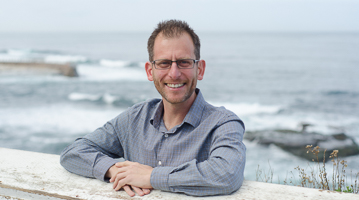
\includegraphics[clip, trim=.1cm 0cm .2cm 0cm,width=.2\textwidth]{../Images/roger.jpg}};
	\end{tikzpicture}
		\begin{tikzpicture}[remember picture,overlay]
	\node[xshift=-2cm,yshift=2cm] at (current page.south east) {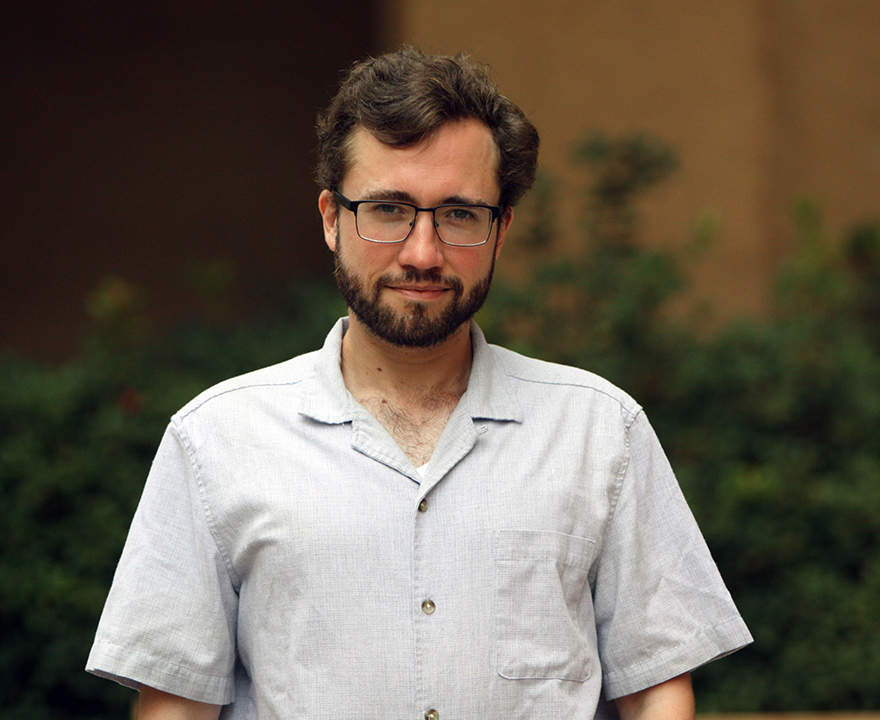
\includegraphics[clip, trim=.1cm 0cm .2cm 0cm,width=.2\textwidth]{../Images/richard.jpg}};
	\end{tikzpicture}
	\begin{tikzpicture}[remember picture,overlay]
	\node[xshift=-2cm,yshift=-2cm] at (current page.north east) {
\includegraphics[width=.3\textwidth]{../Images/cpl_header.png}};
	\end{tikzpicture}
	
\end{frame}
%

\section{Why RT?}
\begin{frame}{Why measure reading time?}
\pause
Linguistic and psycholinguistic theories make predictions about processing difficulty.
\medskip
\pause

Examples of increased difficulty
\begin{itemize}
	\item Constructions not in the grammar 
	\item Lexical items that are harder to retrieve 
	\item Words that force reparsing or reanalysis
\end{itemize}
\pause
\medskip 

We assume that harder processing manifests in longer reading/reaction time (RT).
\pause
\medskip

RT patterns may be phenomena that theories need to explain.




\end{frame}

\begin{frame}{Two common methods}
%can't get at the internals of processing, so want to use time as proxy for how much is going on 
%but literate humans are good at reading 
\begin{columns}[t]\pause
	\begin{column}{.5\textwidth}
		\begin{center}
			\textbf{\Large Eye-tracking}
			
			\medskip
			
			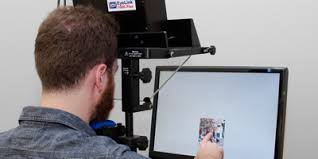
\includegraphics[width=.9\textwidth]{../Images/eye-tracker.jpeg}
			\pause
			\begin{itemize}
				\item Expensive
				\item Hard to analyse
			\end{itemize}
		\end{center}
	\end{column}\pause
	\begin{column}{.5\textwidth}
		\begin{center}
\textbf{\Large Self-paced reading}

\medskip

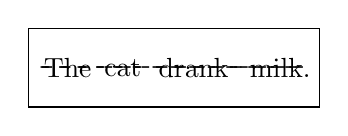
\begin{tikzpicture} 
\draw (-.5,-.5) rectangle (3.2,.5);
\onslide<4>{\node at (0,0) {The};}
\onslide<4>{\node at (1.7,0) {- - - - - - - - - - -};}
\onslide<5>{\node at (0,0) {- - - };}
\onslide<5>{\node at (.7,0) {cat};}
\onslide<5>{\node at (2,0) {- - - - - - - - };}
\onslide<6>{\node at (0.3,0) {- - - - - - };}
\onslide<6>{\node at (1.6,0) {drank};}
\onslide<6>{\node at (2.6,0) {- - - -};}
\onslide<7->{\node at (.9,0) {- - - - - - - - - - -};}
\onslide<7->{\node at (2.7,0) {milk.};}
\end{tikzpicture}
\end{center}
\onslide<8->{
			\begin{itemize}
	\item Lots of spillover
	\item Messy data 
\end{itemize}
}
\end{column}
\end{columns}
	\bigskip
\onslide<9->{Different methods have different trade-offs}
\end{frame}

\begin{frame}[c]{An alternative: Maze}
	
	
	\centering
	
	\bigskip 
	
	\tikzset{
		font={\fontsize{14pt}{12}\selectfont}}
	
\begin{tikzpicture}
	\onslide<1-2>{\node  (c) at (-1,.5) {The};}
	\onslide<1-2>{\node  (d) at (1,.5) {x-x-x};}
	\onslide<3-4>{\node  (c) at (-1,.5) {upon};}
	\onslide<3-4>{\node  (d) at (1,.5) {dog};}
	\onslide<5-6>{\node  (c) at (-1,.5) {revise};}
	\onslide<5-6>{\node  (d) at (1,.5) {chased};}
	\onslide<7-8>{\node  (c) at (-1,.5) {the};}
	\onslide<7-8>{\node  (d) at (1,.5) {wish};}
	\onslide<9-10>{\node  (c) at (-1,.5) {mitigate.};}
	\onslide<9-10>{\node  (d) at (1,.5) {squirrel.};}
	\onslide<2,8>{\node[ultra thick, draw=blue, ellipse, minimum width=60pt, minimum height= 25pt,align=center] at (c) {};}
	\onslide<4,6,10>{\node[ultra thick, draw=blue, ellipse, minimum width=60pt, minimum height= 25pt,
		align=center] at (d) {};}
	\end{tikzpicture}
\end{frame}


\begin{frame}{A third option: Maze}
\begin{columns}
	\begin{column}{0.5\textwidth}
		\begin{center}
		\textbf{\large G-maze}
		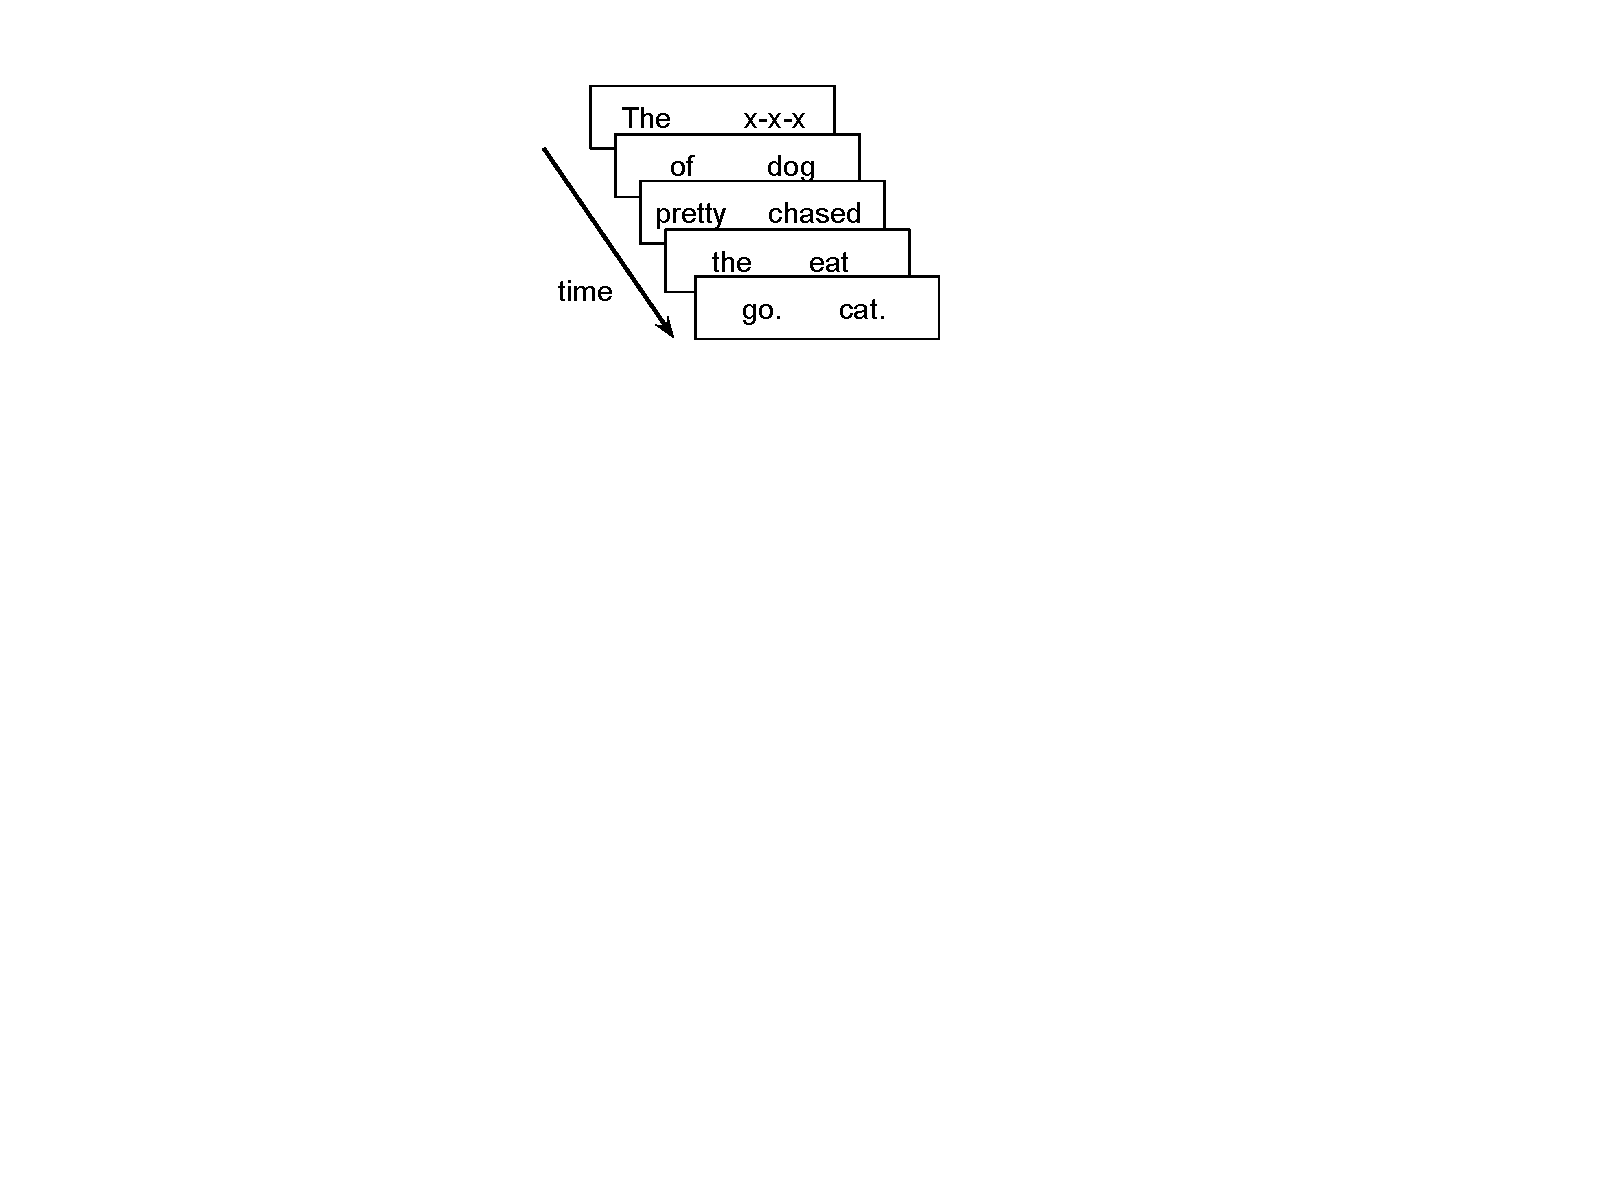
\includegraphics[clip, trim=9cm 14cm 11cm 1cm,width=.9\textwidth]{../Images/gmaze.pdf}
		\end{center}
	\pause
	\end{column}
	\begin{column}{0.5\textwidth} 
		\begin{center}
		\textbf{\large L-maze}
			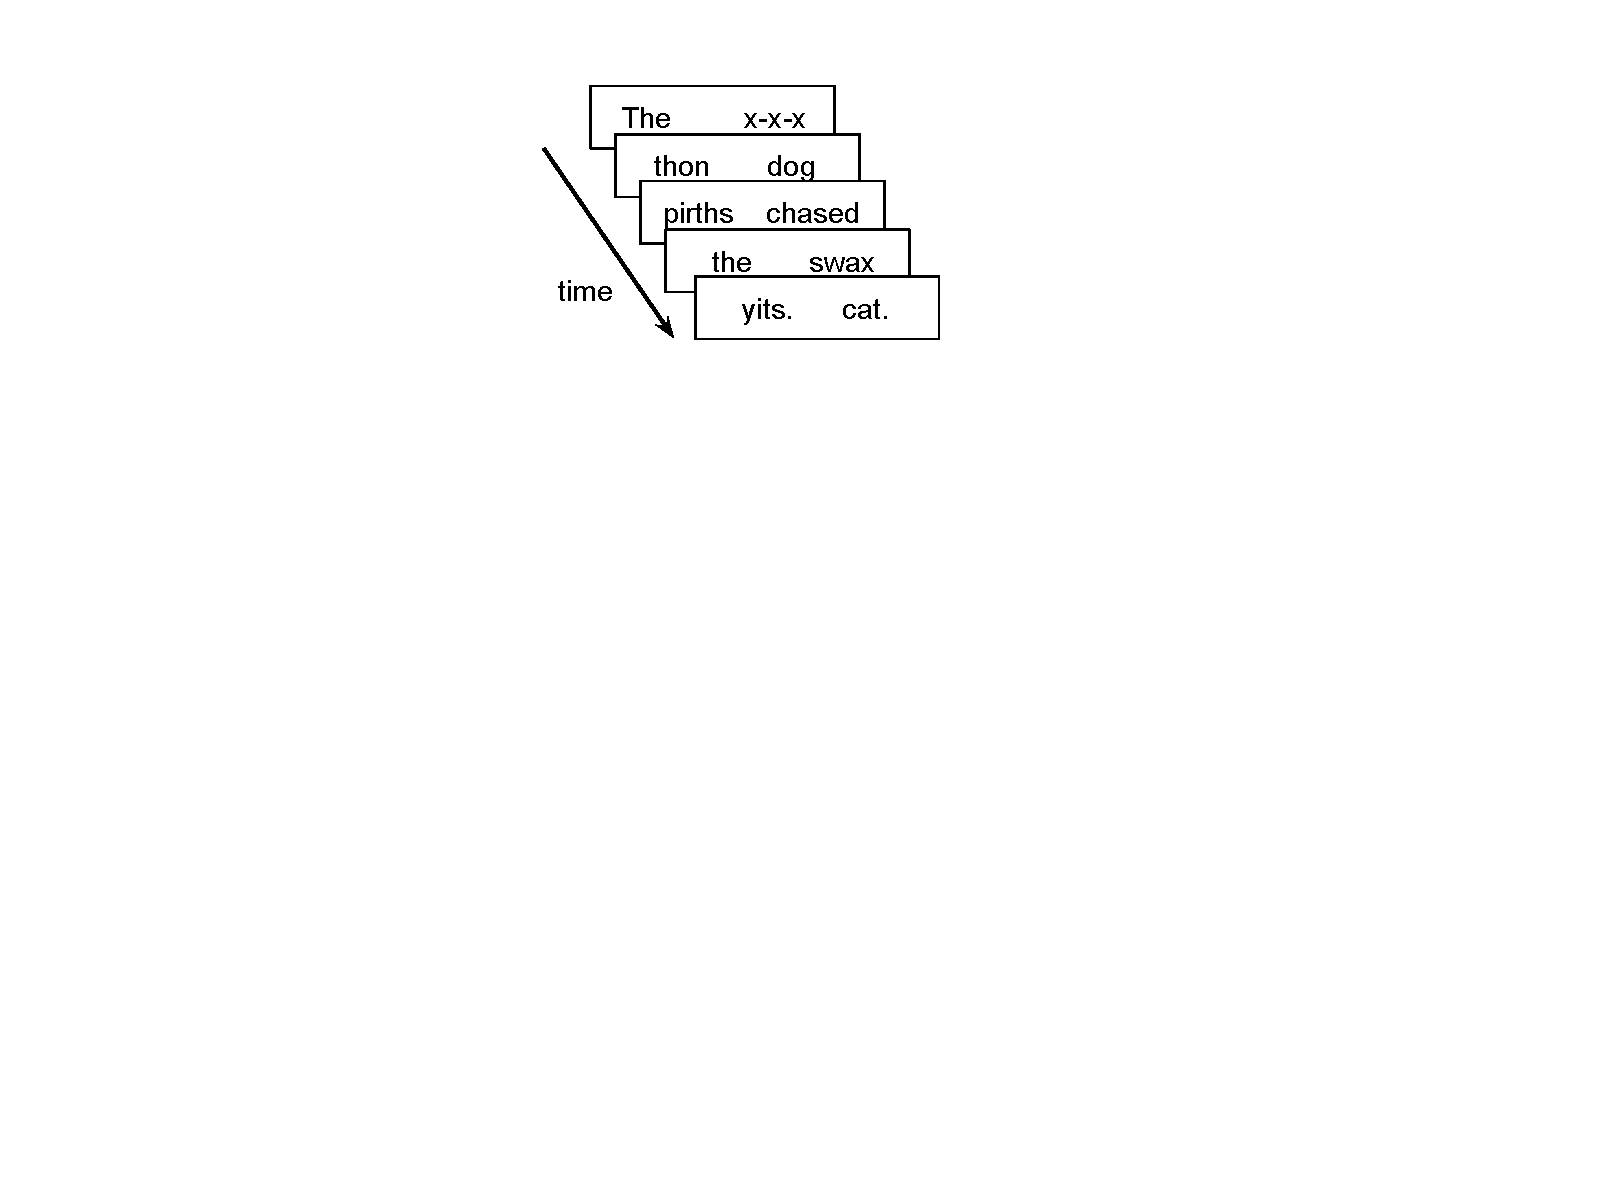
\includegraphics[clip, trim=9cm 14cm 11cm 1cm,width=.9\textwidth]{../Images/lmaze.pdf}
		\end{center}
	\end{column}
\end{columns}

\medskip
\pause
Sentence ends when a mistake is made.
\pause

Central claim: forces extremely incremental processing (no spillover)

\begin{flushright}
	{\small(Forster et al. 2009; Witzel et al. 2012)}
\end{flushright}
\end{frame}

\begin{frame}{Maze Made Easy}
	
	Can we use Maze instead of web SPR?\pause
	
	\medskip
	
	Needs some tweaks:\pause
	\begin{itemize}
		\item Run on web \pause
		\item Easily generate distractors \pause
		\item Work for multi-sentence items
	\end{itemize} 
	
\end{frame}

\section{Experiment 1a}
\begin{frame}{Run on web}
	
	\pause
	\begin{columns}
		\begin{column}{0.5\textwidth}
				Wrote an Ibex module
		\end{column}
		\begin{column}{0.5\textwidth} 
			\begin{center}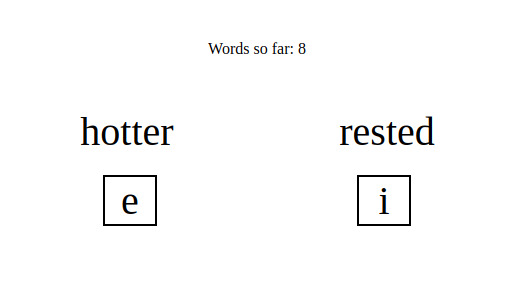
\includegraphics[width=\textwidth]{../Images/screenshot.png} \end{center}\pause
		\end{column}
	\end{columns}

Test by replicating Witzel et al. (2012)
\begin{itemize}
	\item Witzel et al (2012): Comparison of eye-tracking, SPR, L-maze, G-maze (all in-lab)
	\item Got materials and data from Witzel
	\item We run SPR, L-maze, and G-maze on MTurk
\end{itemize}
\end{frame}


\begin{frame}{Materials}

\textbf{Relative Clause}

\sethlcolor{green}
\textit{Low:} The son of the \uline{lady} who politely introduced \hl{herself} was popular at the party.
\sethlcolor{pink}

 \textit{High:} The \uline{son} of the lady who politely introduced \hl{himself} was popular at the party.
 

\textbf{Adverb Clause}

\sethlcolor{green}\textit{Low:} James will fix the car he \uline{drove} \hl{yesterday}, but he will need some help.

\sethlcolor{pink} \textit{High:} James \uline{will fix} the car he drove \hl{tomorrow}, but he will need some help.
		
\textbf{Sentence v Noun Phrase conjunction}

\sethlcolor{green} \textit{Comma:} The swimmer disappointed her \uline{coach}, and her mother \hl{tried} to console her.

\sethlcolor{pink}
\textit{No comma:} The swimmer disappointed her \uline{coach} and her mother \hl{tried} to console her.
\end{frame}

\begin{frame}{Results}
\begin{small}	
	\sethlcolor{green}
The son of the lady who politely introduced \hl{herself}\sethlcolor{pink} / \hl{himself} was popular at the party.
	
\end{small}
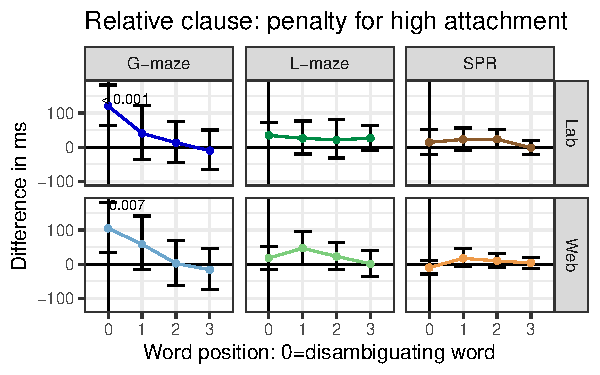
\includegraphics[width=\textwidth]{../Images/g_rel.pdf}
\end{frame}

\begin{frame}{Results}
\begin{small}	

\sethlcolor{green}James will fix the car he drove \hl{yesterday}\sethlcolor{pink} / \hl{tomorrow},  but he will need some help.

\end{small}
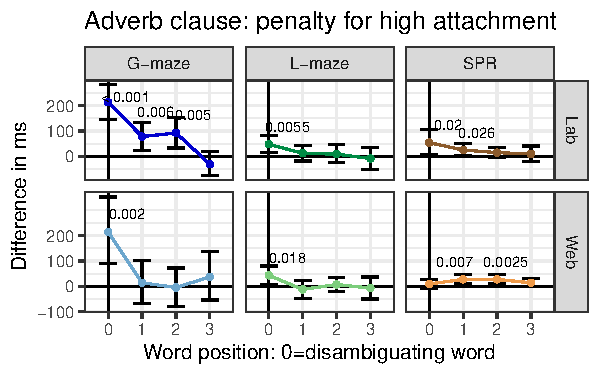
\includegraphics[width=\textwidth]{../Images/g_adv.pdf}
\end{frame}

\begin{frame}{Results}
\begin{small}	
\sethlcolor{green}The swimmer disappointed her coach\hl{,} and her mother \hl{tried} / \sethlcolor{pink}\hl{tried} to console her.
\end{small}
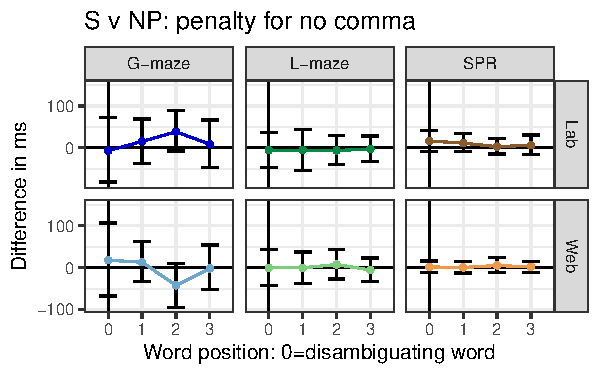
\includegraphics[width=\textwidth]{../Images/g_svnp.pdf}
\end{frame}

\begin{frame}{Maze Made Easy}
	
	Can we use Maze instead of web SPR?
	
	\medskip
	
	Needs some tweaks:
	\begin{itemize}
		\item Run on web \greencheck
		\item Easily generate distractors
		\item Work for multi-sentence items 
	\end{itemize} 
	
\end{frame}

\section{A-maze}

\begin{frame}{Generating distractors}
	\pause
	Goal: Find a word that can't continue a partial sentence
	\begin{itemize}
		\item Ex.  \textit{The dog chased} \pause
		\item Tedious (and hard!) to do by hand
	\end{itemize} \pause
	
	What makes something an unacceptable continuation? \pause
	\begin{itemize}
		\item Ungrammatical \pause
		\item ...or otherwise really unlikely \pause 
		\item $\approx$ high surprisal 
	\end{itemize} \pause
	
	Can we use Neural Language Models?
\end{frame}

\begin{frame}{Meanwhile in Natural Language Processing}
\pause
Language models (LMs)
\begin{itemize}
	\item Trained on large corpora to predict the next word
	\item Given a partial sentence, return probabilities of the next word
\end{itemize}
Surprisal: negative log probability
\begin{itemize}
	\item 2 bits of surprisal = 1/4
	\item 10 bits of surprisal $\approx$ 1/1000 
	\item +1 surprisal = half as likely
\end{itemize}
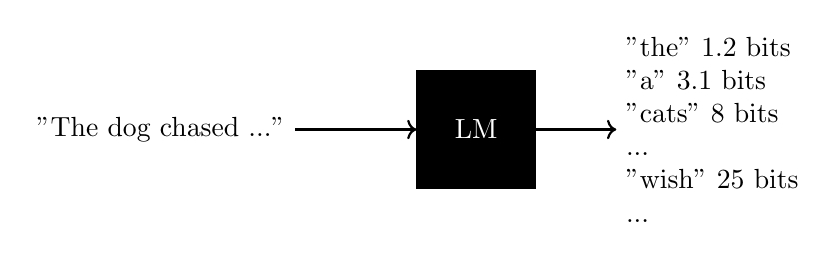
\begin{tikzpicture}
\node (A) at (0,0) {"The dog chased ..."};
\node  (B) at (4,0) [draw, minimum width=1.5cm, minimum height=1.5cm, fill=black] {\textcolor{white}{LM}} ;
\draw [->, thick] (A) -- (B); 
\node[align=left] (C) at (7,0) {"the" 1.2 bits \\"a" 3.1 bits\\"cats" 8 bits\\...\\"wish" 25 bits\\...};
\draw [->, thick] (B) -- (C); 
\end{tikzpicture}
\end{frame}

\begin{frame}{Can we use LMs to choose distractors?} 
	
	Use high surprisal according to LM as a proxy for bad in context
	\medskip
	
	\pause
	
	\begin{itemize}
		\item Model the target sentence word by word \pause
		\item At each position, choose a high surprisal word
	\end{itemize}
	\medskip
	\pause
	Want quality control on distractors
	\pause
	\begin{itemize}
		\item Restrict to a list of possible distractors \pause
		\item Only consider distractors of same length, frequency as target word \pause
		\item Check distractors until we find one with high surprisal
	\end{itemize}
	
\end{frame}

\begin{frame}
	\centering
	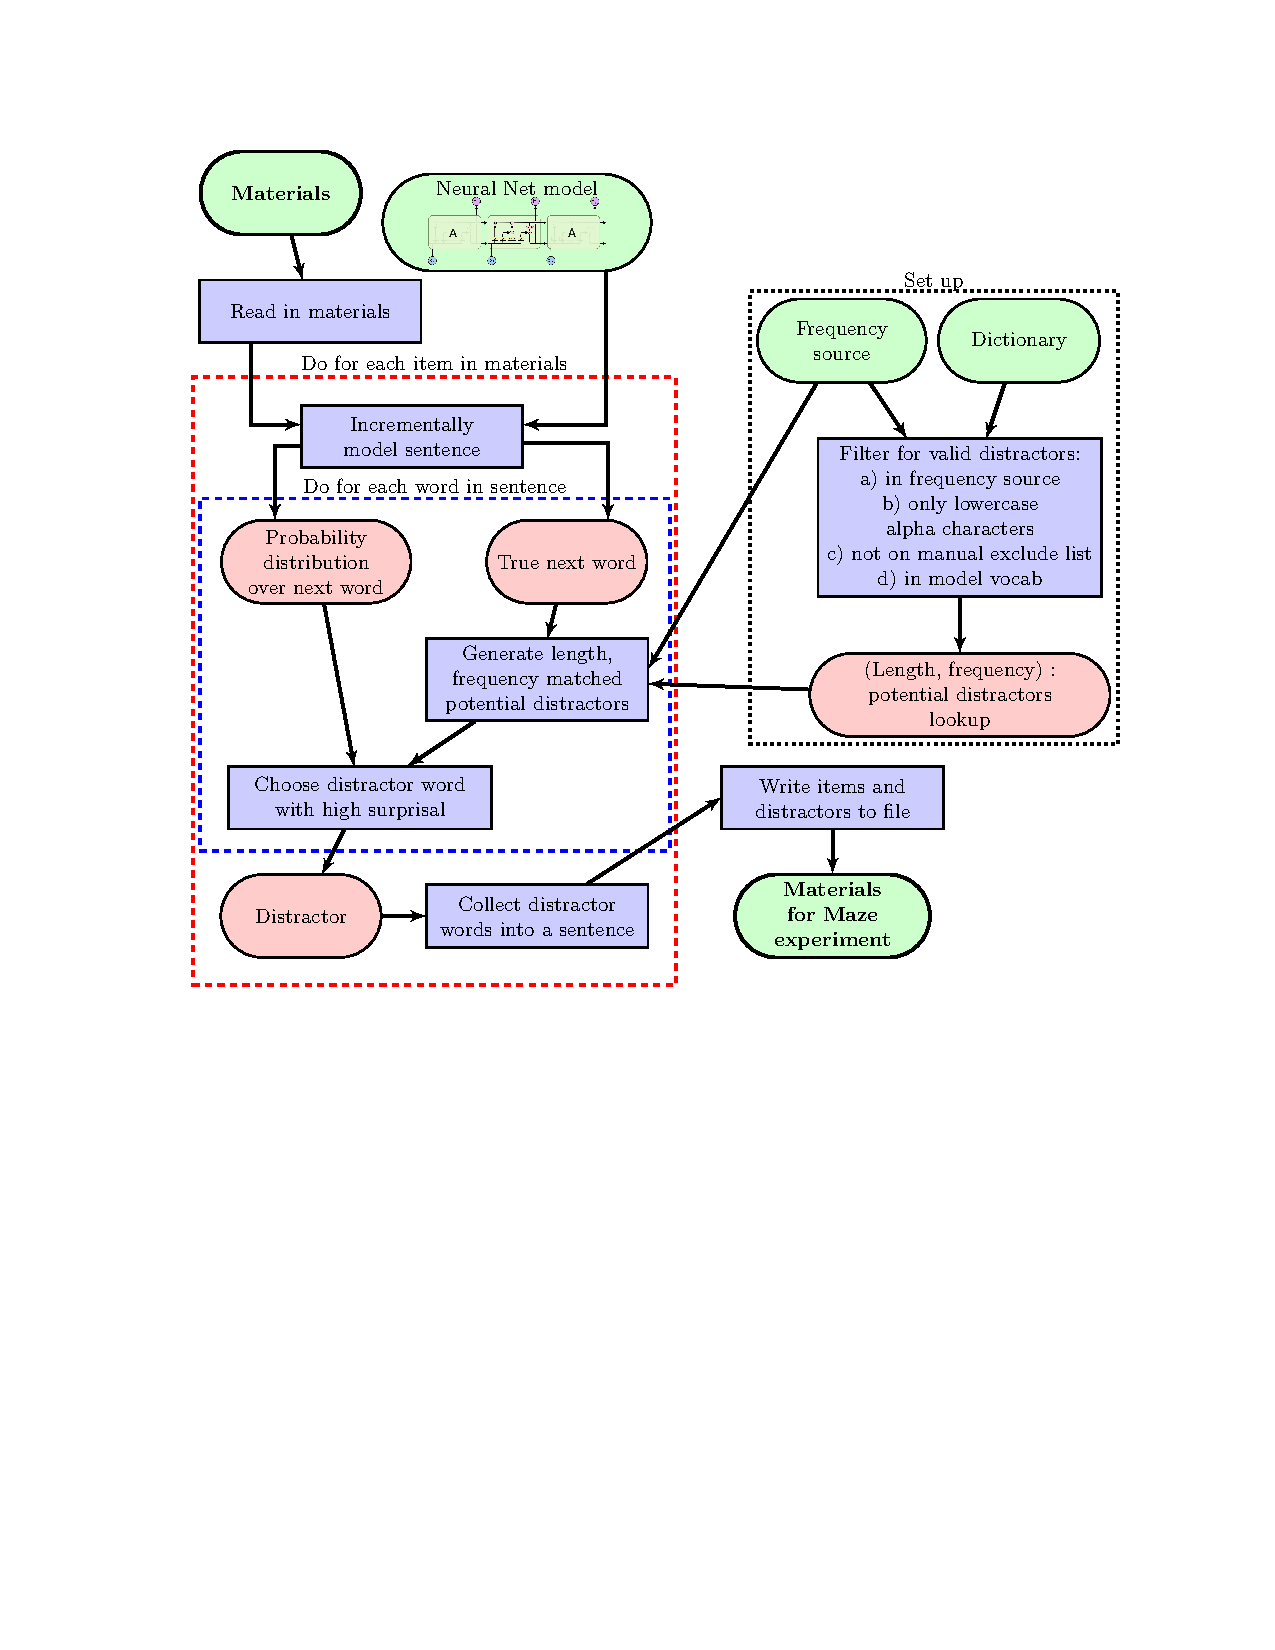
\includegraphics[clip, trim=3.25cm 5cm 2.5cm 2.5cm,width=.9\textwidth]{../Images/flow_2.pdf}
\end{frame}


\section{Experiment 1b}


\begin{frame}{Does it work?} 
	%\vskip -2em
	\medskip
	
	\centering
	
	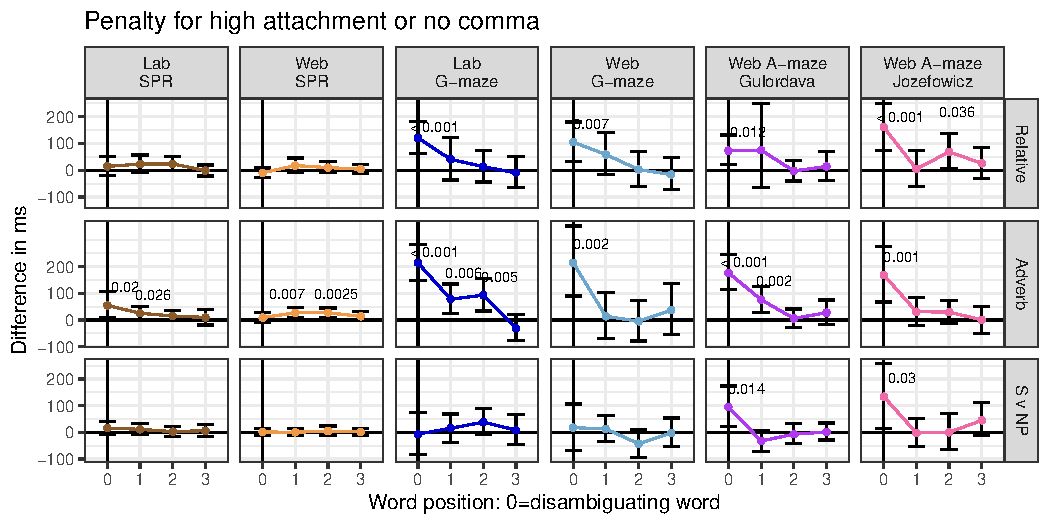
\includegraphics[width=\textwidth]{../Images/spr_g_amaze.pdf}
	
	{\footnotesize Error bars: 95\% CI}
	
\end{frame}

\begin{frame}{Does it work?} 
	\pause
	%\vskip -2em
	{\large Yes, at least well enough.} \pause
	\begin{itemize}
		\item Caveat: Sometimes generates plausible distractors. \pause
		\item Sloggett et al (2020) also found A-maze results comparable with G-maze
	\end{itemize} 
\end{frame}

\section{Error-correction A-Maze}

\begin{frame}{Maze Made Easy}
	
	Can we use Maze instead of web SPR?
	
	\medskip
	
	Needs some tweaks:
	\begin{itemize}
		\item Run on web \greencheck
		\item Easily generate distractors \greencheck
		\item Work for multi-sentence items 
	\end{itemize} 
	
\end{frame}

\begin{frame}{Long items}

	Want to run multi-sentence items. \pause
	
	Problem: Errors terminate sentences. \pause
	\begin{itemize}
		\item Treat whole story as a unit: \pause Few participants make it to the end. \pause
		\item Treat each sentence as a unit: \pause Some participants miss key context. \pause
		
	\end{itemize}
	
	What if after an error, participants corrected errors and the sentence continued?
	
\end{frame}

\begin{frame}[c]{Maze with Error Correction}
	\centering
	\tikzset{
		font={\fontsize{14pt}{12}\selectfont}}
	
	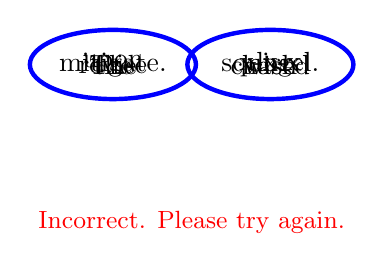
\begin{tikzpicture}
	\onslide<1-2>{\node  (c) at (-1,.5) {The};}
	\onslide<1-2>{\node  (d) at (1,.5) {x-x-x};}
	\onslide<3-4>{\node  (c) at (-1,.5) {upon};}
	\onslide<3-4>{\node  (d) at (1,.5) {dog};}
	\onslide<5-8>{\node  (c) at (-1,.5) {revise};}
	\onslide<5-8>{\node  (d) at (1,.5) {chased};}
	\onslide<9-10>{\node  (c) at (-1,.5) {the};}
	\onslide<9-10>{\node  (d) at (1,.5) {wish};}
	\onslide<11-12>{\node  (c) at (-1,.5) {mitigate.};}
	\onslide<11-12>{\node  (d) at (1,.5) {squirrel.};}
	\onslide<2,6,10>{\node[ultra thick, draw=blue, ellipse, minimum width=60pt, minimum height= 25pt,align=center] at (c) {};}
	\onslide<4,8,12>{\node[ultra thick, draw=blue, ellipse, minimum width=60pt, minimum height= 25pt,
		align=center] at (d) {};}
	\onslide<7,8>{\node[text=red] at (0,-1.5) {\small Incorrect. Please try again.};}
	\end{tikzpicture}
	
\end{frame}

\begin{frame}{Maze with Error Correction}
	
%	Incidentally, also ``solves'' problem of bad distractors!
	
	\begin{columns}
		\begin{column}{0.4\textwidth}
			\begin{center}
				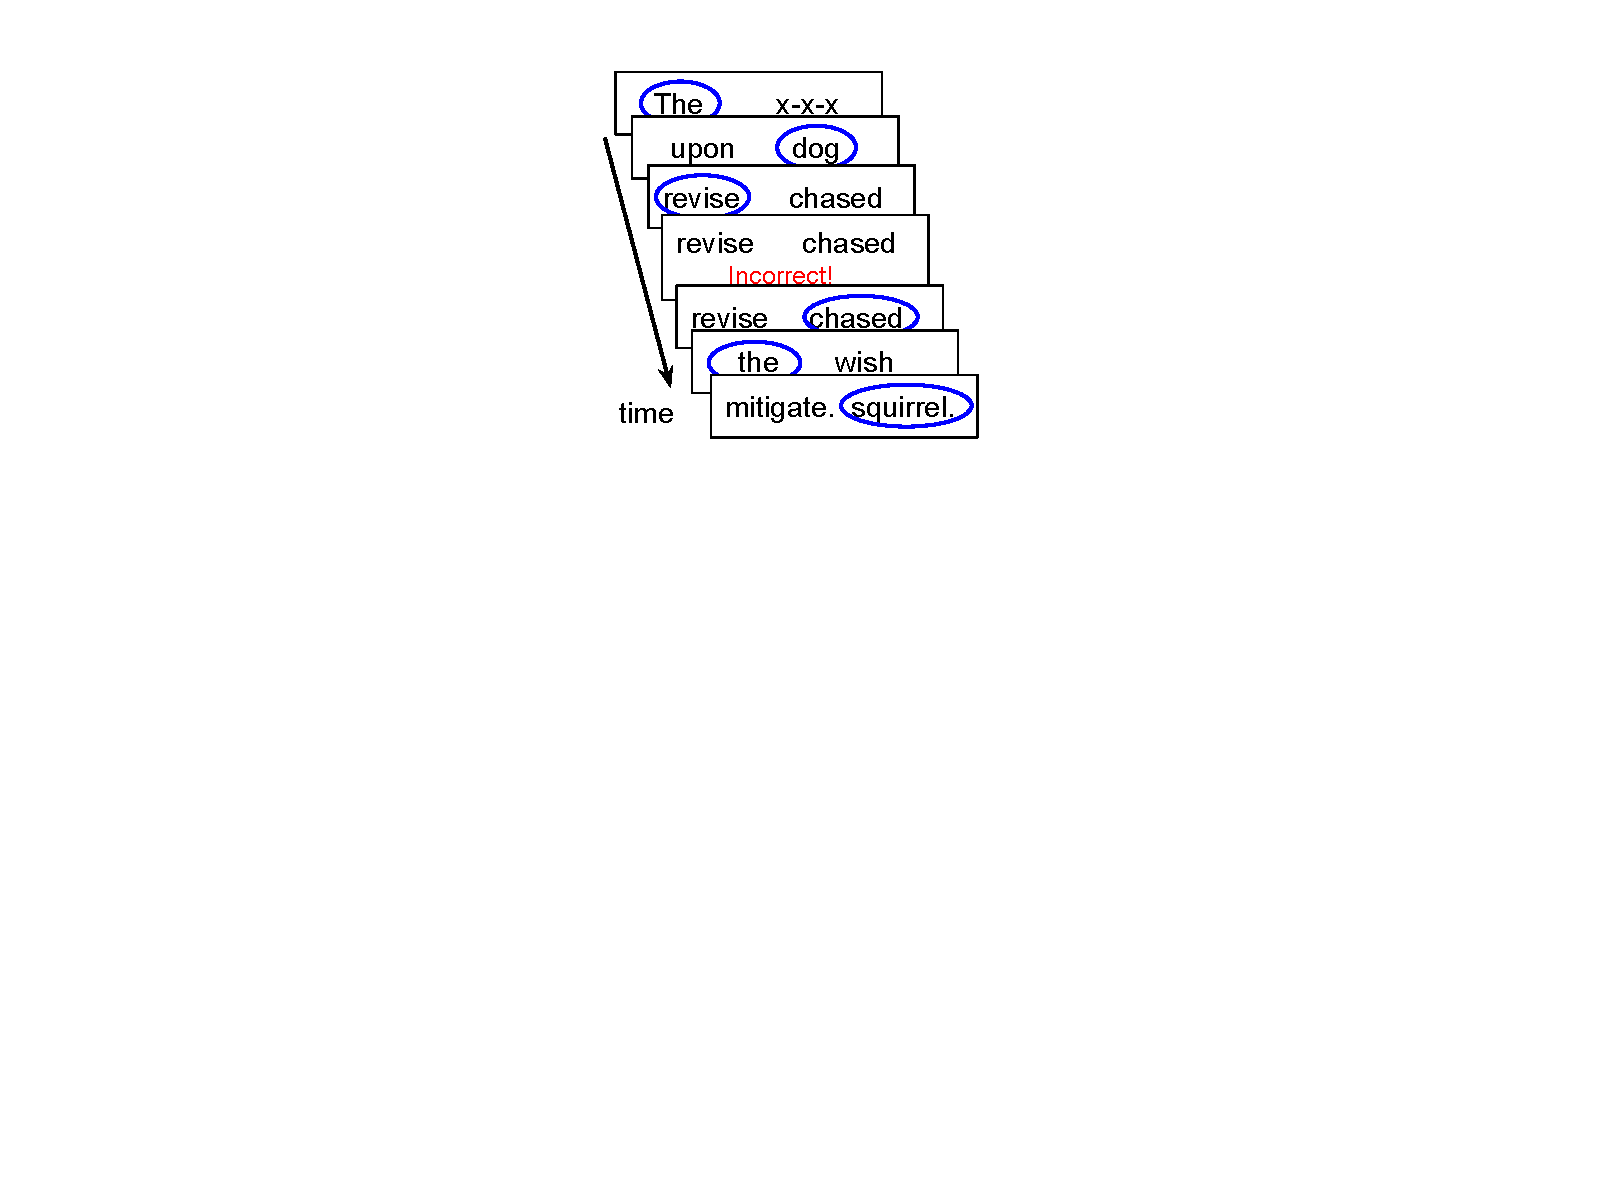
\includegraphics[clip, trim=9cm 12.5cm 10cm 1cm,width=\textwidth]{../Images/maze_diagram.pdf}
			\end{center}
			
		\end{column} \pause 
		\begin{column}{0.6\textwidth} 
			\begin{center}
				\begin{itemize}
					\item Can be toggled in Ibex Maze \pause
					\item Long materials feasible \pause
					\item Have all the data \pause
					\item Compensates for bad distractors
				\end{itemize}
			\end{center}
		\end{column}
	\end{columns}
\end{frame}
%
\begin{frame}{Maze Made Easy}
	
	Can we use Maze instead of web SPR?
	
	\medskip
	
	Needs some tweaks:
	\begin{itemize}
		\item Run on web \greencheck
		\item Easily generate distractors \greencheck
		\item Work for multi-sentence items \greencheck ? 
	\end{itemize} 
	
\end{frame}

\section{Experiment 2}
\begin{frame}{}
	Various open questions to address \pause
	\begin{itemize}
		\item Will people read long texts in Maze? \pause
		\item Will they comprehend what they read? \pause
		\item Does error correction Maze work? \pause
		\item Do we get predictability effects? 
	\end{itemize}
\end{frame}

\begin{frame}{Natural Stories}
	Natural stories corpus (Futrell et al. 2017) \pause
	\begin{itemize}
		\item 10 stories, each about 1000 words \pause
		%	\item Some unusual constructions, but read fluently \pause
		\item 6 comprehension questions per story
	\end{itemize}
	
\end{frame}


\begin{frame}{Natural Stories}

\begin{small}Tulip mania was a period in the Dutch Golden Age during which contract prices for bulbs of the recently introduced tulip reached extraordinarily high levels and then suddenly collapsed. At the peak of tulip mania in February sixteen thirty-seven, tulip contracts sold for more than ten times the annual income of a skilled craftsman. It is generally considered the first recorded economic bubble. [...]
\medskip

Q: When did tulip mania reach its peak?

A: \hspace{3em} 1630's\hspace{3em} 1730's \end{small}

\end{frame}


\begin{frame}{Participant accuracy}
100 participants each read 1 story \pause
\begin{center}
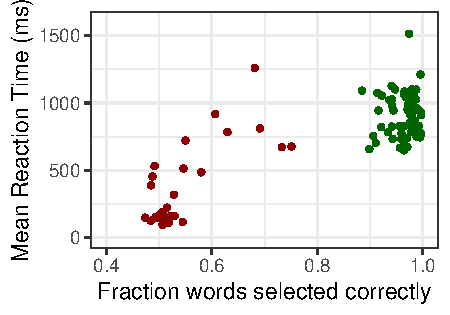
\includegraphics[width=.8\textwidth]{../Images/error.pdf}
\end{center}
\end{frame}
\begin{frame}{Comprehension questions}
\begin{center} \pause
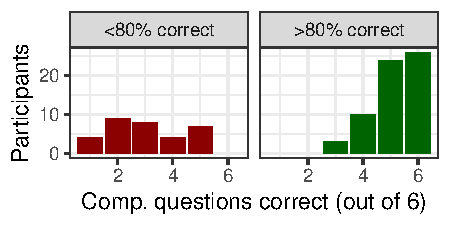
\includegraphics[width=.8\textwidth]{../Images/comp.pdf}
\end{center}
\end{frame}



\begin{frame}{Surprisal Effects}
	\large{Is RT linear in terms of surprisal?}\pause
	\medskip
	
	Estimate surprisal from 3 models:
	\begin{itemize}
		\item smoothed 5-gram
		\item LSTM-RNN (Gulordava et al. 2018)
		\item Transformer-XL (Dai et al. 2019)
	\end{itemize}
	
	\pause
	
	Fit GAMs
	\begin{itemize}
		%\item Limit to single-token words
		\item Fit to both current and past word surprisal
		\item Include frequency, length as predictors
	\end{itemize}
	
\end{frame}



\begin{frame}{Surprisal Effects}
	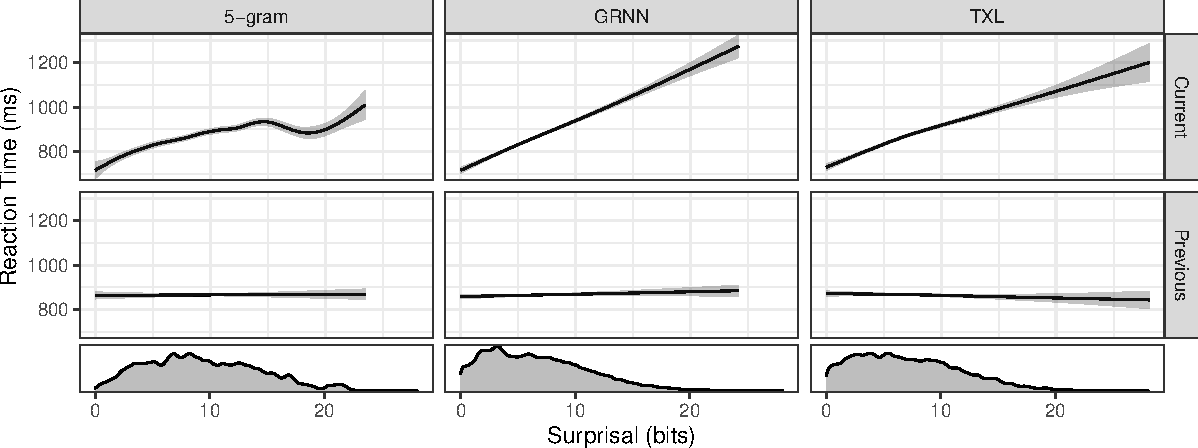
\includegraphics[width=\textwidth]{../Images/amaze_gam.pdf}	
\end{frame}


\begin{frame}{SPR comparison}
	Using SPR data collected by Futrell et al. (2017)
	
	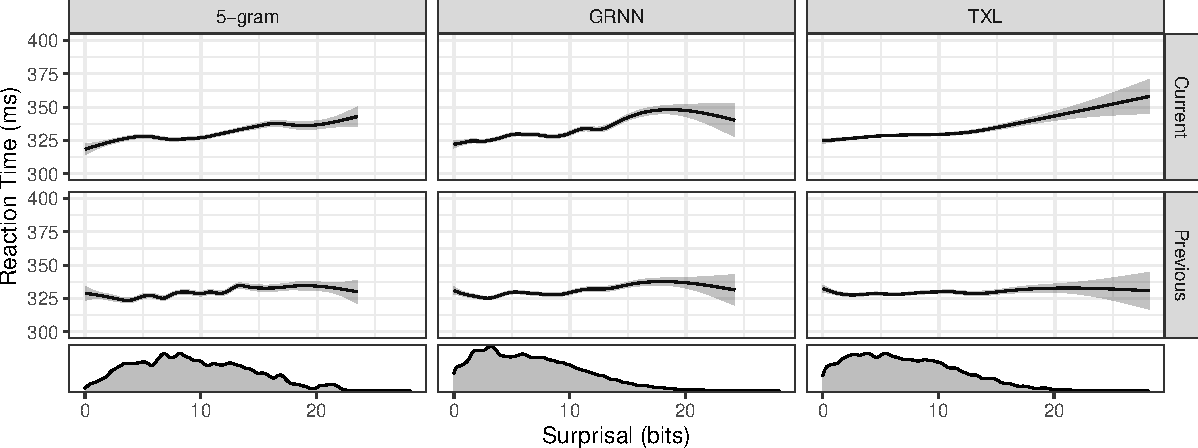
\includegraphics[width=\textwidth]{../Images/spr_gam.pdf}
	
\end{frame}

\begin{frame}{Surprisal Effects}
	\vskip -2em
	Linear Models \\ 
	\pause
	
	\begin{small}
		\begin{tabular}{l|r|r|r}
			\hline
			&5-gram & GRNN & TXL\\
			\hline
			Intercept & \textbf{865.3} & \textbf{871.1} & \textbf{870.8} \\ 
			Surprisal & \textbf{11.7}  & \textbf{23.7} & \textbf{18.5}  \\ 
			Frequency & -2.9  & 2.9  & 0.4  \\ 
			Length & \textbf{20.5} & \textbf{18.5}  & \textbf{21.4} \\ 
			Surprisal:Length & \textbf{-2.0}  & \textbf{-1.8}  & \textbf{-1.4} \\
			Freq:Length & -1.0  & -0.1 & 0.2  \\ 
			\hline
			Past Surprisal & 1.6  & \textbf{2.7} & 0.8 \\ 
			Past Freq & 2.6  & 1.9  & 1.2  \\ 
			Past Length & \textbf{-4.8}  & \textbf{-6.6 }&\textbf{ -5.2} \\ 
			Past Surp:Length & -0.2 & \textbf{-0.9} & -0.6  \\ 
			Past Freq:Length & -1.0  & \textbf{-1.8 }&   \textbf{-1.5}  \\ 
			\hline
		\end{tabular}
		
		Surprisal in bits, Length in characters, \\
		Frequency in $log_2$ occurrences/billion words
	\end{small}
	
\end{frame}
\begin{frame}{Surprisal Effects}
	Takeaways: 
	\begin{itemize}
		\item Minimal frequency effects (consistent with Shain 2019) 
		\item Large effects of Length, Surprisal
		\item Very little spillover 
	\end{itemize}
	%	
%	Model comparison: GRNN is best, but TXL complementary
\end{frame}

\begin{frame}{Summary}
	\begin{itemize}\pause
		\item People will read in the Maze task for 15-20 minutes \pause
		\item It's possible to comprehend during Maze \pause
		\item Distractors are generally good enough \pause
		\item Find expected RT patterns \pause
		\item Very little spillover
	\end{itemize}
\end{frame}

\section{Conclusion}

\begin{frame}{Consider A-maze!}
Easy to use! \pause
\begin{itemize}
	\item Runs on command line \pause
	\item Match distractors across minimal pair sentences \pause
	\item Customize surprisal thresholds, vocabulary lists \pause
	\item Can output pre-formatted for Ibex\pause
\end{itemize}

Adapt A-maze to your projects:
\begin{itemize}
	\item Written in Python 3 
	\item Interface with other language models 
	\item Add more frequency sources 
	\item Extend to non-English languages
\end{itemize}
\medskip
\end{frame}


\begin{frame}{}

\textcolor{ForestGreen}{\large Documentation: vboyce.github.io/Maze}

with links to the following:
\begin{itemize}

\item A-maze code: github.com/vboyce/Maze

\item Web-maze code: github.com/vboyce/Ibex-with-Maze

\item Exp 1 Paper: psyarxiv.com/b7nqd/
\end{itemize}
\end{frame}


\appendix

\begin{frame}{Matching distractors}
If unspecified: Match by position
\begin{itemize}
	\item The son of the lady who politely introduced \sethlcolor{green} \hl{herself}\sethlcolor{pink} / \hl{himself} was popular at the party.
\end{itemize}
Can specify labels for each word to pair (within item)
\begin{itemize}
	\item The cat who the dog scared hid in a box.\\pre-1 pre-2 who art noun verb main-verb post-1 post-2 post-3
\item The dog who scared the cat sniffed around the couch.\\ pre-1 pre-2 who verb art noun main-verb post-1 post-2 post-3
\end{itemize}
\end{frame}


\begin{frame}{Regression coefficients}
\begin{tiny}
\begin{tabular}{l|rlr|rlr|rlr}
	\hline
	&\multicolumn{3}{c|}{5-gram}&\multicolumn{3}{c|}{GRNN}&\multicolumn{3}{c}{TXL}\\
	& Est & CI & $p$ & Est & CI & $p$ &Est & CI & $p$ \\ 
	\hline
	Intercept & 865.3 & [829.9, 902.9] & 0.00 & 871.1 & [837.9, 905.3] & 0.00 & 870.8 & [832.5, 907.8] & 0.00 \\ 
	Surprisal & 11.7 & [9.3, 14.1] & 0.00 & 23.7 & [21, 26.5] & 0.00 & 18.5 & [16.1, 21.1] & 0.00 \\ 
	Frequency & -2.9 & [-6.3, 0.5] & 0.10 & 2.9 & [-0.2, 6] & 0.06 & 0.4 & [-2.7, 3.5] & 0.79 \\ 
	Length & 20.5 & [15.4, 25.6] & 0.00 & 18.5 & [13.3, 23.7] & 0.00 & 21.4 & [16.2, 26.6] & 0.00 \\ 
	Surprisal:Length & -2.0 & [-3, -1] & 0.00 & -1.8 & [-2.7, -0.9] & 0.00 & -1.4 & [-2.2, -0.6] & 0.00 \\
	Freq:Length & -1.0 & [-2.5, 0.4] & 0.16 & -0.1 & [-1.2, 1] & 0.82 & 0.2 & [-0.9, 1.2] & 0.76 \\ 
	\hline
	Past Surprisal & 1.6 & [-0.5, 3.6] & 0.14 & 2.7 & [0.8, 4.5] & 0.00 & 0.8 & [-0.9, 2.5] & 0.40 \\ 
	Past Freq & 2.6 & [-0.1, 5.4] & 0.06 & 1.9 & [-0.2, 4.2] & 0.08 & 1.2 & [-1.1, 3.6] & 0.30 \\ 
	Past Length & -4.8 & [-9, -0.1] & 0.04 & -6.6 & [-10.9, -2.1] & 0.00 & -5.2 & [-9.3, -0.7] & 0.03 \\ 
	Past Surp:Length & -0.2 & [-1.2, 0.8] & 0.72 & -0.9 & [-1.7, -0.2] & 0.01 & -0.6 & [-1.3, 0.2] & 0.13 \\ 
	Past Freq:Length & -1.0 & [-2.3, 0.3] & 0.15 & -1.8 & [-2.9, -0.8] & 0.00 & -1.5 & [-2.6, -0.5] & 0.01 \\ 	
	\hline
\end{tabular}
\end{tiny}
\end{frame}


\begin{frame}{Caveats}
	
	{\large Definitely some bad distractors}
	\begin{table}
		
		
		\begin{tabular}{rlll}
			Prefix & Correct & Distractor & Error Rate \\
			\hline
			\hline
			Gulordava&&&\\
			\hline
			The & niece & cooks & 44\%\\
			The swimmer & disappointed & propositions & 30\%\\
			The & semester & steroids & 29\%\\
			\hline
			\hline
			Jozefowicz&&&\\
			\hline
			The & husband & authors & 46\%\\
			Jim & listened & survived & 43\%\\
			The & uncle & roads & 42\%\\
			The & knight & saints & 40\%\\
		\end{tabular}
	\end{table}
	
\end{frame}


\begin{frame}{What about post-mistake data?}
	Exclude data from mistakes or the two words after a mistake. 
	
	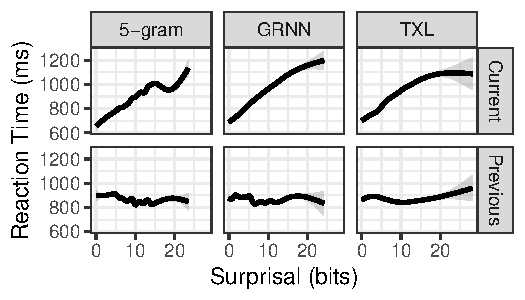
\includegraphics[width=.9\textwidth]{../Images/gam2.pdf}	
\end{frame}

\begin{frame}{Why such large effects?}
	Bayesian Reader (Norris 2006): Look at words long enough to ID with some threshold of certainty 
	
	
	Possible mechanisms for difference: 
	\begin{itemize}
		\item Higher threshold 
		\item Fewer available resources for processing
		\item Presence of second word 
	\end{itemize}
	
\end{frame}
\end{document}

